% ROME student lab procedure (Plan 3 Task 5, spec Part G). DRAFT.
% Packages are limited to the Plan 3 set. Run check_procedure.py (python -I -X utf8) after every edit.
% Provenance rules for this file:
%   * every number in the student part (before \appendix) is on number_allowlist.tsv with a
%     file:line citation, or sits inside \todo{BLOCKED: ...} / \todo{NOT VERIFIED: ...};
%   * \src{path:lines} cites the code or lab document behind a statement. The PRINTED citations name
%     only files of the lab repository layout (paths relative to UK-Simulink-v3/, the model folder, or
%     to the repository root for UK-Arduino/);
%   * a source that is a review document (TRACKER.md, the plans, run logs, CLAUDE.md, the manuscript)
%     is cited on a comment line of its own whose text starts with the word review-src and a colon,
%     then path:lines entries separated by semicolons. check_procedure.py resolves and locks these
%     in the review folder and lists them as review-only in the repo;
%   * every TRACKER.md section 0 row has a "% tracker: <key>" line in Section 11.
% COMPILED (19 Nov, doc pass): MiKTeX pdflatex (%LOCALAPPDATA%\Programs\MiKTeX\miktex\bin\x64), twice, and once
% more if the log says Rerun, in a copy of this folder; the PDF is beside this file as ROME_lab_procedure.pdf.
% Rebuild it the same way after every edit.
\documentclass[11pt]{article}
\usepackage{graphicx}
\usepackage{amsmath}
\usepackage{siunitx}
\usepackage{enumitem}
\usepackage{booktabs}
\usepackage{tikz}
\usepackage{hyperref}

\setlength{\textwidth}{6.5in}
\setlength{\oddsidemargin}{0in}
\setlength{\evensidemargin}{0in}
\setlength{\textheight}{9in}
\setlength{\topmargin}{-0.5in}
\setlength{\parindent}{0pt}
\setlength{\parskip}{4pt}
% Extra stretch so a line before a long unbreakable word is set loose instead of running into the margin.
\setlength{\emergencystretch}{3em}
\hypersetup{colorlinks=true, linkcolor=blue, urlcolor=blue}

% ---------------------------------------------------------------- macros
% \todo marks what is not measured, not built or not verified yet. xcolor comes with tikz.
\newcommand{\todo}[1]{\textcolor{red}{\textbf{[#1]}}}
% Code text printed as it is, character by character (like \detokenize), with a permitted line break after
% / _ ; : , . so that a long path or name does not run into the margin (doc pass, 19 Nov: a citation ran
% 155 pt past the right edge of the page). expl3 is part of the LaTeX kernel; no package is added.
\ExplSyntaxOn
\cs_new_protected:Npn \romecode #1
  {
    \str_map_inline:nn {#1}
      {
        ##1
        \str_if_in:nnT { /_;:,. } {##1} { \penalty 50 \relax }
      }
  }
\ExplSyntaxOff
% Something the student types, or a name in the code, printed as it is.
\newcommand{\cmd}[1]{\texttt{\romecode{#1}}}
% A line MATLAB prints.
\newcommand{\out}[1]{\texttt{\romecode{#1}}}
% Source of a statement. Set \showsrcfalse to hide the sources in a print for students.
\newif\ifshowsrc
\showsrctrue
\newcommand{\src}[1]{\ifshowsrc{\scriptsize\,[\texttt{\romecode{#1}}]}\fi}
% The result a step should give.
\newcommand{\expect}{\par\textit{Expected result.}\ }
% A boxed warning.
\newcommand{\warn}[1]{\par\medskip\noindent\fbox{\parbox{\dimexpr\linewidth-2\fboxsep-2\fboxrule\relax}{\textbf{Warning.} #1}}\par\medskip}
% Numbered steps, numbered within the section (5.3 is step 3 of Section 5).
\newlist{steps}{enumerate}{1}
\setlist[steps]{label=\thesection.\arabic*, leftmargin=*, itemsep=3pt}
% Troubleshooting entries.
\newlist{trouble}{enumerate}{1}
\setlist[trouble]{label=T\arabic*, leftmargin=*, itemsep=4pt}
\newcommand{\sym}{\textbf{Symptom.}\ }
\newcommand{\act}{\par\textbf{What to do.}\ }
% Column widths of the table of modes (set here so that no number sits in the body).
\newlength{\modehead}
\setlength{\modehead}{0.13\textwidth}
\newlength{\modecol}
\setlength{\modecol}{0.18\textwidth}

\title{ROME robot\\Student lab procedure}
\author{Spacecraft simulation laboratory}
\date{DRAFT, 19 November 2026. Not for use on the robot.}

\begin{document}
\maketitle

\warn{This is a draft. Red text marks a value that is not measured, a tool that is not built
yet, or a result that is not verified. A step that carries a red BLOCKED note cannot be done
yet. The hardware sections, Sections~\ref{sec:calib} to~\ref{sec:save}, stay closed to students
until the TA has signed what Table~\ref{tab:modes} lists for the mode: the whole bench checklist,
its joint-map test included, before any robot run, mode 2 included, and the lab-frame checklist
for the mode with the cameras on (Section~\ref{sec:setup}).}
% review-src: TRACKER.md section 2, 19 Nov "Q-P4-a answered"

How to read this procedure. Do the sections in order. Each step is one action. After a step that
checks something, the expected result is given. If you see something else, stop and look the
symptom up in Section~\ref{sec:trouble}. Sources are given in small brackets, for the TA. All
paths are inside the model folder \cmd{UK-Simulink-v3} of the lab repository.

\tableofcontents

% =====================================================================================
\section{Before you start}\label{sec:start}

\subsection*{What the robot does}
ROME is a ground vehicle with four wheels that carries a six-joint arm
\src{define_constants.m:128; define_constants.m:201}. In a run, the computer commands only the
tool at the end of the arm, the end effector. The end effector follows a path that reproduces the
motion of a spacecraft relative to a target, scaled down to the floor. The controller decides
how the base and the arm share that motion \src{define_constants.m:17-22; define_constants.m:49-58}.
The base therefore drives over the floor during a run, and the arm moves on top of it.

The same model runs in four modes, listed in Section~\ref{sec:modes}. You choose the mode with one
number, \cmd{run_mode}. In simulation nothing is sent to the robot. In a robot run the model sends
wheel speeds and joint angles to the robot over the robot's wireless network
\src{run_mode_table.m:5; docs/lab/PART_C_LAB_VISIT.md:86}.

\subsection*{Safety rules}
\begin{steps}
  \item Read Section~\ref{sec:stop} (Stopping) before you touch the robot.
  \expect You can name the three ways to stop the robot and the order in which to use them.
  \item Find the physical power cut-off of the robot.
  \todo{BLOCKED: location of the power cut-off, Part F item 25c and photo C13\_18\_estop\_location.jpg}
  \expect You can reach it without walking into the robot's area.
  \item Work in pairs. During every motion one person keeps a hand on the power cut-off and the
  other person is at the keyboard \src{docs/lab/PART_F_BENCH_CHECKLIST.md:18}.
  \item Keep the clear zone around the arm empty while the arm has power
  \src{docs/lab/PART_F_BENCH_CHECKLIST.md:20}.
  \todo{BLOCKED: clear-zone radius, from the measured reach of the arm (Part F item 24d) plus the margin the author sets}
  \item Stay clear below the arm when the power is cut. Whether the arm holds or falls without
  power is not known \src{docs/lab/PART_F_BENCH_CHECKLIST.md:21}.
  \todo{BLOCKED: arm behaviour on power loss, Part F item 25c}
  \item Leave \cmd{run_mode} at mode 1, simulation only, unless the TA has opened
  Section~\ref{sec:hw} for you \src{run_mode_table.m:30}.
  \expect The line reads \cmd{run_mode = 1;} \src{define_constants.m:7}.
\end{steps}

\subsection*{The three ways to stop}
Use them in this order. Section~\ref{sec:stop} gives the details.
% review-src: TRACKER.md section 0, row 19 Nov "Arm does not stay stopped after STOP_ALL"
\begin{enumerate}[label=(\alph*)]
  \item Press \textbf{Stop} in Simulink. Stopping the model sends the stop command
  \cmd{STOP_ALL} to the robot \src{ROMECommand.m:194-196}.
  \item Send \cmd{STOP_ALL}. Never send a bare \cmd{!}. The robot ignores it when it comes from MATLAB
  \src{UK-Arduino/ROME_ESP32_Code/ROME_ESP32_Code.ino:141-147}.
  \todo{BLOCKED: a tested student command that sends STOP\_ALL on its own (the Part F snippets are NOT RUN)}
  \item Cut the power. During arm calibration this is the only way to stop the arm
  \src{UK-Arduino/ROME_Teensy_Code/ROME_Teensy_Code.ino:160-163}.
\end{enumerate}

% =====================================================================================
\section{One-time lab setup (TA)}\label{sec:setup}
The TA does this section once, before any student uses the robot. It refers to the two lab
checklists and does not repeat them \src{docs/lab/PART_C_LAB_VISIT.md; docs/lab/PART_F_BENCH_CHECKLIST.md}.

\begin{steps}
  \item Install MATLAB R2026a with Simulink on the lab PC. Students run the model on that PC with
  that release. An older release fails in the checks (Section~\ref{sec:trouble}).
% review-src: TRACKER.md section 2, 19 Nov "Lab PC, R2026a"; TRACKER.md section 0, row 19 Nov "derivation_checks fails on R2025a"
  \expect Typing \cmd{version} in MATLAB prints a version that contains \out{R2026a}.
  \todo{BLOCKED: lab PC name and installed toolboxes, not recorded yet}
  \item Copy the model folder \cmd{UK-Simulink-v3} of the lab repository to the lab PC.
  \todo{BLOCKED: the repository branch that carries this procedure, after the port}
  \expect The folder holds \cmd{define_constants.m}, \cmd{ROME_9DOF.slx} and a \cmd{tests} folder.
  \item Run the test suite once on the lab PC, as Appendix~\ref{app:suite} describes.
  \expect The last line reads \out{test_suite PASS: ... steps, define_constants.m unchanged}
  \src{tests/test_suite.m:128}.
  \todo{BLOCKED: the lab PC run is done only after all tests on the author's PC are done}
  \item Carry out the lab-frame checklist \cmd{docs/lab/PART_C_LAB_VISIT.md} and sign it. Only
  mode 4, cameras on, needs it.
  \todo{BLOCKED: lab visit, and the origin of the floor frame}
% review-src: TRACKER.md section 3, Q-D2
  \expect Its sign-off table is complete and signed.
  \item Carry out the bench checklist \cmd{docs/lab/PART_F_BENCH_CHECKLIST.md} in the order it
  gives, and sign it \src{docs/lab/PART_F_BENCH_CHECKLIST.md:29}. Its joint-map test settles the
  J2, J5 and J6 maps of the arm
  \src{docs/lab/PART_F_BENCH_CHECKLIST.md:180; docs/lab/PART_F_BENCH_CHECKLIST.md:192}. The whole
  checklist, its joint-map test included, is signed before any robot run, mode 2 included,
  although mode 2 keeps the arm parked. There is no partial sign-off
  \src{docs/lab/PART_F_BENCH_CHECKLIST.md:277}.
% review-src: TRACKER.md section 2, 19 Nov "Q-P4-a answered"; TRACKER.md section 3, Q-P4-a
  \todo{BLOCKED: bench session at the lab}
  \expect Its sign-off table is complete and signed, and a signed copy is saved where the checklist
  says \src{docs/lab/PART_F_BENCH_CHECKLIST.md:5}.
  \item Enter both sign-off dates in the sign-off file.
  \todo{BLOCKED: lab\_signoff.m does not exist yet}
  \item Connect the lab PC to the robot's wireless network and to the camera stream.
  \todo{BLOCKED: how one PC reaches both networks, open question for the lab}
% review-src: TRACKER.md section 3, Q-L2
  \item Tape the floor frame and the start mark of every case, as the lab-frame checklist
  describes in its item C11 \src{docs/lab/PART_C_LAB_VISIT.md:179-194}.
  \expect The marks match Figure~\ref{fig:frame} and the Part C photographs.
\end{steps}

% =====================================================================================
\section{Frame and floor marks}\label{sec:frame}
All positions on the floor are given in the floor frame of Figure~\ref{fig:frame}. Its origin is
the target. The $x$ axis points radially, the $y$ axis in-track, and $z$ up. The heading
$\theta_v$ of the base is measured from $+x$, counter-clockwise seen from above
\src{define_constants.m:34-36}. The start card prints the heading as
\out{yaw}, in degrees \src{define_constants.m:426-427}.
% review-src: docs/2026-11-18-rome-sim-to-lab-plan.md:49

\begin{figure}[h]
  \centering
  % Top view of the floor frame for ROME_lab_procedure.tex (Plan 3 Task 5).
% Schematic, not to scale. No measured value is drawn: the origin location (TRACKER Q-D2), the
% tracked region (Part C C9.6) and the start marks (Part C C11) are not measured yet.
% Frame: spec docs/2026-11-18-rome-sim-to-lab-plan.md step 10 (origin = target, x radial,
% y in-track, z up, heading from +x). Heading symbol theta_v from Research/writing_rules/NOTATION.md
% (the task brief wrote psi, which NOTATION.md reserves for the constraint function).
% Drawn x right, y up, so that z up points out of the page (right-handed), CLAUDE.md section 28.
\begin{tikzpicture}[>=stealth]
  % tracked region, not measured
  \draw[dashed, gray] (-3.4,-2.2) rectangle (3.4,2.2);
  \node[gray, anchor=north west, font=\footnotesize] at (-3.35,2.15) {tracked region (Part C, not yet measured)};
  % floor frame
  \draw[->, thick] (0,0) -- (2.4,0) node[right] {$x$ radial};
  \draw[->, thick] (0,0) -- (0,1.7) node[above] {$y$ in-track};
  \draw (0,0) circle (0.13);
  \fill (0,0) circle (0.045);
  \node[anchor=north west, font=\footnotesize, align=left] at (0.1,-0.1) {origin at the target\\$z$ up, out of the page};
  % schematic robot at a start pose
  \begin{scope}[shift={(-1.9,-1.0)}, rotate=35]
    \draw[thick, fill=gray!15] (-0.35,-0.35) rectangle (0.35,0.35);
    \draw[->, thick] (0,0) -- (0.8,0) node[right, font=\footnotesize] {heading};
  \end{scope}
  \draw[dotted] (-1.9,-1.0) -- (-0.8,-1.0);
  \draw[->] (-1.35,-1.0) arc (0:35:0.55);
  \node[font=\footnotesize] at (-1.05,-0.78) {$\theta_v$};
  \node[font=\footnotesize, align=center] at (-1.9,-1.75) {start pose of your case\\(printed on the card)};
\end{tikzpicture}

  \caption{Top view of the floor frame. Schematic, not to scale.}
  \label{fig:frame}
\end{figure}

\todo{BLOCKED: where the origin is in the room}
% review-src: TRACKER.md section 3, Q-D2
\todo{BLOCKED: Part C photo C13\_02\_floorplan\_topview.jpg}

\begin{steps}
  \item Find the origin mark on the floor.
  \todo{BLOCKED: Part C photo C13\_03\_origin\_tape.jpg}
  \expect A taped mark that matches the photograph.
  \item Find the $+x$ axis line that starts at the origin.
  \todo{BLOCKED: Part C photo C13\_04\_xaxis\_tape.jpg}
  \expect A tape line from the origin, labelled $+x$.
  \item Find the $+y$ axis line.
  \todo{BLOCKED: Part C photo C13\_05\_yaxis\_tape.jpg}
  \expect The $+y$ line is at a right angle to the $+x$ line, a quarter turn counter-clockwise
  from it seen from above.
  \item Find the start mark of your case.
  \todo{BLOCKED: Part C photos C13\_06\_case1\_start\_pose.jpg to C13\_10\_case5\_start\_pose.jpg}
  \expect A taped position for the base and a heading line, labelled with the case.
  \item Leave the tape as it is. If a mark is missing or loose, stop and tell the TA. Taping is
  part of the lab-frame checklist \src{docs/lab/PART_C_LAB_VISIT.md:179-194}.
\end{steps}

% =====================================================================================
\section{Constants you may change}\label{sec:const}
You change the robot's settings in one place only. That place is the top block of the file
\cmd{define_constants.m}, between the line \out{EDIT THIS BLOCK. NOTHING ELSE IN THIS FILE NEEDS TOUCHING.}
and the line \out{Below here is the formulation. Leave it alone.}
\src{define_constants.m:2; define_constants.m:171}.

The run mode is one of these constants, \cmd{run_mode} (Section~\ref{sec:modes}). The settings that
say whether the robot is commanded, where the base pose comes from and whether the arm is parked
follow from it. You do not type them \src{run_mode_table.m:13-14; define_constants.m:12-13; define_constants.m:177; define_constants.m:179-182}.

Table~\ref{tab:const} lists every constant you may change, with its meaning, unit, default value,
allowed range and the source of the range.

\begin{table}[h]
  \centering
  \caption{Constants you may change.}
  \label{tab:const}
  \IfFileExists{generated/constants_table.tex}{\input{generated/constants_table.tex}}{\todo{BLOCKED: generated by Step 1 (a tools script reads allowed\_ranges.m, which is not written yet)}}
\end{table}

\begin{steps}
  \item Open the file. In MATLAB, in the model folder, type \cmd{edit define_constants}.
  \expect The editor shows the file. Its first lines are the banner \out{EDIT THIS BLOCK.}
  \src{define_constants.m:1-3}.
  \item Change only the constants listed in Table~\ref{tab:const}. Change nothing below the
  second banner.
  \item Do not type a constant in the Command Window instead. The file sets every constant again
  each time it runs, so a value typed in the Command Window is lost
  \src{define_constants.m:5; docs/lab/PART_C_LAB_VISIT.md:46}. Never type \cmd{EnableHardware},
  \cmd{EnableMotive}, \cmd{motive_source} or \cmd{arm_freeze}: a Run whose settings differ from the
  run mode is refused with a message that says \out{the run flags do not match run_mode}
  \src{arm_freeze_banner.m:76-79}.
  \item Save the file, then type \cmd{define_constants}. A run refuses to start when
  \cmd{define_constants.m} was changed after it last ran \src{arm_freeze_banner.m:54-55}.
  \expect The editor tab shows no unsaved-change mark, and MATLAB prints the mode line and the
  start card.
  \item Before a robot run, the pre-run check compares every value with its allowed range.
  \todo{BLOCKED: pre-run check, not built yet}
  \expect A value outside its range is refused, and the message names the value, its range and
  the source of the range.
\end{steps}

% =====================================================================================
\section{Run the simulation}\label{sec:sim}

\subsection*{The four modes}\label{sec:modes}
Case 1, the elliptical orbit, runs in four modes. Table~\ref{tab:modes} lists them, in the
author's words \src{run_mode_table.m:16-20}. You choose one with a single line of
\cmd{define_constants.m}, \cmd{run_mode = n;} with $n$ the mode \src{define_constants.m:7}. You can
also type \cmd{rome_mode(n)}, or press the button \textbf{Mode n} on the canvas of the model. The
command and the buttons change that line for you and run \cmd{define_constants} again
\src{define_constants.m:14-15; rome_mode.m:2-3; rome_mode.m:11-17; tools/wire_run_mode_buttons.m:7}.
Each run of \cmd{define_constants} prints the mode line \src{define_constants.m:183}, and
\cmd{rome_mode} prints it once more, last, after \out{rome_mode:} \src{rome_mode.m:51}. A number
other than 1 to 4 is refused with a message that lists the four modes \src{define_constants.m:175-176}.
At every Run the model prints the mode line again
\src{arm_freeze_banner.m:120}, so the Command Window always tells you the mode of the run. The label
on the canvas names the mode that the last button or \cmd{rome_mode} set. Saving the model resets the
label to a text that names no mode, so after the model is opened again only the mode line tells
the mode \src{run_mode_label.m:5-8; tools/wire_run_mode_buttons.m:19}. While the model runs, the
command and the buttons refuse to change the mode; let the run end or press \textbf{Stop} first
\src{rome_mode.m:22-24}.
\todo{NOT VERIFIED: a click on a Mode button has not been tested (a click cannot be made in a test without the screen); the buttons' text and callback are read back by the wiring tool}
% review-src: docs/superpowers/plans/2026-11-19-case1-three-modes.md:60-65

Camera off means the fake camera: no camera is used, and the model sends its own predicted base
pose through the same software path that the camera data take, so the controller receives a
pose in the same form as from the real cameras, but nothing measures where the real base is
\src{run_mode_table.m:7; define_constants.m:42}.

Start with mode 1, which is this section. Modes 2, 3 and 4 are Section~\ref{sec:hw}, in that
order. Mode 2 is the first student robot run. This procedure describes modes 2 to 4 for case 1 only.
% review-src: docs/superpowers/plans/2026-11-19-case1-three-modes.md:14-28; TRACKER.md section 2, 19 Nov "First student robot run: base only, camera off"

\begin{table}[!htbp]
  \centering
  \small
  \caption{The four modes of case 1. Each mode is one value of \cmd{run_mode} in
  \cmd{define_constants.m}.}
  \label{tab:modes}
  \begin{tabular}{p{\modehead}p{\modecol}p{\modecol}p{\modecol}p{\modecol}}
    \toprule
    & \textbf{Mode 1} & \textbf{Mode 2} & \textbf{Mode 3} & \textbf{Mode 4} \\
    In the author's words & Simulation only (end-effector dynamics sim, pose data from sim) &
      ground vehicle moving, frozen arm, camera off (pose data from sim) & ground vehicle moving,
      moving arm, camera off (pose data from sim) & ground vehicle moving, moving arm, camera on \\
    \midrule
    What moves & Nothing. Only the model runs. & The base, along the base path of the full plan
      of base and arm. The arm stays parked at its start posture, and the end effector is not
      tracked. & The base and the arm. & The base and the arm. \\
    \addlinespace
    Base pose from & The fake camera, with simulated camera noise
      \src{define_constants.m:89; define_constants.m:332}. & The fake camera, no noise
      \src{define_constants.m:305}. & The fake camera, no noise. & The OptiTrack cameras,
      converted to the floor frame: where the robot really is
      \src{define_constants.m:33-37; Optitrack/motive_to_floor.m:34; Optitrack/motive_to_floor.m:39-40}. \\
    \addlinespace
    Arm angles the controller reads & The model's own. & The model's own: with the arm frozen
      the controller uses its model of the arm \src{tools/wire_motive_emulator.m:70}. &
      The real arm, as it reports its joint angles. & The real arm, as in mode 3. \\
    \addlinespace
    Set with & \cmd{run_mode = 1;} (the default) & \cmd{run_mode = 2;} & \cmd{run_mode = 3;} &
      \cmd{run_mode = 4;} \\
    \addlinespace
    Signed off first & Nothing. & The whole bench checklist (Part F), its joint-map test
      included, as for every robot mode. No lab frame, no taped marks. & The whole bench checklist,
      as for mode 2, with the J2, J5 and J6 maps of its joint-map test. & As mode 3, plus the lab-frame checklist
      (Part C) with the camera calibration. Refused until the calibration is measured
      \src{define_constants.m:38-42}. \\
    \bottomrule
  \end{tabular}
\end{table}
% The author's words are run_mode_table.m:17-20, with "movinb" written "moving" as in the banners.
% review-src: run_mode_table.m:29-33; docs/superpowers/plans/2026-11-19-case1-three-modes.md:15-18; docs/superpowers/plans/2026-11-19-case1-three-modes.md:21-26
% review-src: TRACKER.md section 2, 19 Nov "Mode 2 is the base-path test, as built"; TRACKER.md section 2, 19 Nov "Q-P4-a answered"

\subsection*{Mode 1, simulation only}\label{sec:mode1}
This section is mode 1 of Table~\ref{tab:modes}. It needs only MATLAB. Nothing is sent to the robot.

\begin{steps}
  \item Start MATLAB R2026a.
% review-src: TRACKER.md section 2, 19 Nov "Lab PC, R2026a"
  \expect Typing \cmd{version} prints a version that contains \out{R2026a}.
  \item Change to the model folder with \cmd{cd}.
  \todo{BLOCKED: path of the model folder on the lab PC}
  \expect Typing \cmd{pwd} prints the path of that folder.
  \item Type \cmd{edit define_constants}. In the line \cmd{scenario = 1;}, set the number to
  your case. The comment on the same line lists the cases, \out{1 ellipse | 2 V-bar | 3 R-bar | 4 NMC | 5 circle}
  \src{define_constants.m:5}.
  \item Set the run mode. In the line \cmd{run_mode = 1;} keep the number 1, or type
  \cmd{rome_mode(1)}, or press \textbf{Mode 1} on the model's canvas.
  \item Save the file and type \cmd{define_constants}. Skip this step if you used
  \cmd{rome_mode} or a button: they run it for you.
  \expect The mode line reads \out{MODE 1: Simulation only (end-effector dynamics sim, pose data from sim)}
  \src{run_mode_table.m:30}. If it names another mode, set \cmd{run_mode = 1;} and repeat.
  \item Check that Fast Restart is off in the Simulink toolstrip. It is refused in every mode,
  simulation included \src{apply_pacing.m:68-70}.
  \item Type \cmd{check_9dof} \src{check_9dof.m:1}. It runs the model for the case you set, in
  mode 1 only: it stops with an error if the run mode is not 1 \src{check_9dof.m:4-5}. That
  message names the mode it found, says \out{Set run_mode = 1 (type rome_mode(1) or press Mode 1)}
  and, after a robot mode, names the command that sets that mode back afterwards
  \src{assert_sim_mode.m:35-42}.
  \expect MATLAB prints the orbit parameters and a card headed \out{PLACE THE ROBOT LIKE THIS},
  then \out{9-DOF VERIFICATION  -  simulation only, no hardware}, two lines that start with
  \out{static: [OK]}, six result lines that start with \out{[OK]}, and finally
  \out{RESULT: PASS} \src{check_9dof.m:58; check_9dof.m:88-89; check_9dof.m:256}.
% review-src: 2026-11-19_p2t1_test_suite.log:7-116
  When the model starts it prints the mode line again, then a line that begins
  \out{*** ARM FROZEN} \src{arm_freeze_banner.m:120}. In mode 1 that second line is
  about the robot only: nothing is sent to it, and the simulated arm moves as usual
  \src{arm_freeze_banner.m:140; run_mode_table.m:25-26}.
  For the elliptical orbit and the circle at the default size MATLAB also prints the warning
  \out{The orbit exceeds a 2m x 2m area! Check dist_scale or a.} That warning is expected and the
  check still passes \src{define_constants.m:440}.
% review-src: TRACKER.md section 0, row 19 Nov (final review) "define_constants prints"; 2026-11-19_p2t1_test_suite.log:43; 2026-11-19_p2t1_test_suite.log:116
  \todo{NOT VERIFIED: how long the run takes on the lab PC}
  \item If you kept the default values of Table~\ref{tab:const}, compare the numbers that
  \cmd{check_9dof} printed with the row of your case in Table~\ref{tab:expected}. The table holds
  the values of the paper's results table. With other values the numbers differ, and only
  \out{RESULT: PASS} counts. The table is for simulation only, never for a robot run
  (Section~\ref{sec:save}).
% review-src: ../Submission/initialSubmission_V3.tex:455-472
  \expect Each value agrees with the table within the tolerance the table gives for it.
  \todo{BLOCKED: tolerance per column, set by the Step 1 script (the residual agrees only at round-off level)}
  \item Type \cmd{plot_9dof} \src{plot_9dof.m:1}. Like \cmd{check_9dof}, it runs in mode 1 only
  \src{plot_9dof.m:36}.
  \expect A set of figures opens. One of them is named \out{9-DOF actuators and solve health - <case name>},
  and the Command Window prints \out{... figures from plotting.m on end-effector quantities,}
  \src{plot_9dof.m:85; plot_9dof.m:114-115}.
  \todo{NOT VERIFIED: plot\_9dof has no saved run log, the cold-read test (Step 4) checks it}
  \item Compare the path figure with Figure~\ref{fig:expected}.
  \expect Success: \out{RESULT: PASS}, and the end-effector path lies on the reference path.
\end{steps}

\begin{table}[h]
  \centering
  \caption{Expected results of the simulation, per case.}
  \label{tab:expected}
  \IfFileExists{generated/expected_results.tex}{\input{generated/expected_results.tex}}{\todo{BLOCKED: generated by Step 1 (a tools script writes the paper's Table 3 values and the gate values per case)}}
\end{table}

\begin{figure}[h]
  \centering
  \IfFileExists{figures/fig_9dof_case_1_path.pdf}{\includegraphics[width=0.48\linewidth]{figures/fig_9dof_case_1_path.pdf}}{\todo{BLOCKED: expected path figure, case 1, drawn by Step 0}}
  \IfFileExists{figures/fig_9dof_case_2_path.pdf}{\includegraphics[width=0.48\linewidth]{figures/fig_9dof_case_2_path.pdf}}{\todo{BLOCKED: expected path figure, case 2, drawn by Step 0}}
  \IfFileExists{figures/fig_9dof_case_3_path.pdf}{\includegraphics[width=0.48\linewidth]{figures/fig_9dof_case_3_path.pdf}}{\todo{BLOCKED: expected path figure, case 3, drawn by Step 0}}
  \IfFileExists{figures/fig_9dof_case_4_path.pdf}{\includegraphics[width=0.48\linewidth]{figures/fig_9dof_case_4_path.pdf}}{\todo{BLOCKED: expected path figure, case 4, drawn by Step 0}}
  \caption{Expected paths on the floor, one panel per case. The circle case has no expected figure.}
  \label{fig:expected}
\end{figure}
% provenance: fig_9dof_cases.m:10-11 (file names), fig_9dof_cases.m:33 (cases 1-4 only, the circle is not in the paper).

% =====================================================================================
\section{Arm calibration}\label{sec:calib}
\warn{Closed until the TA has signed the bench checklist (Section~\ref{sec:setup}). Calibration
drives every joint into its limit switch. Nothing you type stops it. Only the power cut does
\src{UK-Arduino/ROME_Teensy_Code/ROME_Teensy_Code.ino:160-163}.}
% review-src: TRACKER.md section 0, row 19 Nov "Nothing but the power cut"

\begin{steps}
  \item Place the robot first, as Section~\ref{sec:place} describes. The card gives the order: set the
  run mode first, then place the base, then calibrate the arm \src{define_constants.m:430}. Calibrate
  after the last change of \cmd{define_constants.m} (Section~\ref{sec:hwprep}).
  \item Check that the clear zone around the arm is empty and that your partner has a hand on the
  power cut-off.
  \item Connect the lab PC to the robot's wireless network.
  \todo{BLOCKED: network name and procedure, open question for the lab}
% review-src: TRACKER.md section 3, Q-L2
  \item In MATLAB, in the model folder, type \cmd{calibrateROMEArm} \src{calibrateROMEArm.m:1}.
  \expect MATLAB prints \out{Scenario <n> start posture, firmware degrees}, then \out{Connected.}
  and \out{Sending CAL_ARM...} \src{calibrateROMEArm.m:30; calibrateROMEArm.m:52; calibrateROMEArm.m:75}.
  Each joint drives to its limit switch and then to the start posture.
  \todo{NOT VERIFIED: the motion is described from the code, it has not been observed in this campaign}
  \item Read the limit-switch lines. They have the form \out{Joint <k> hit its limit switch!}.
  The number counts from zero, so add one to get the joint, and \out{Joint 1} means J2
  \src{calibrateROMEArm.m:93}.
% review-src: TRACKER.md section 0, row 19 Nov "calibrateROMEArm prints"
  \item Wait for the end of the printout. The script waits at most \SI{120}{\second} for the arm
  \src{calibrateROMEArm.m:11}.
  \expect The last line reads \out{ROME arm calibration successfully completed.}
  \src{calibrateROMEArm.m:205}.
  \item Read the table of joints that the script prints before that line.
  \expect No line that starts \out{DO NOT run a robot mode} \src{calibrateROMEArm.m:192}.
  If that line appears, stop and tell the TA. Do not move joints yourself.
  \item Compare the arm with the posture that the script describes under \out{Expected posture}
  \src{calibrateROMEArm.m:189-190}.
  \todo{BLOCKED: photograph of the calibrated arm in its start posture (not in the Part C photo list)}
  \todo{BLOCKED: the joint map of J2 is not measured, Part F item 24b}
% review-src: TRACKER.md section 0, row 19 Nov "model-firmware map for J2"
  \expect The arm looks like the description. If it does not, stop and tell the TA.
  \item Keep the calibration log. The script writes a file named \out{calib_log_<date>_<time>.csv}
  next to itself \src{calibrateROMEArm.m:74}.
  \item If you had to cut the power, the arm must be calibrated again before any run. After
  power-up the arm reports that it is not calibrated
  \src{UK-Arduino/ROME_Teensy_Code/ROME_Teensy_Code.ino:52}.
\end{steps}

% =====================================================================================
\section{Placement}\label{sec:place}
\warn{Modes 2 and 3 need no lab-frame sign-off. Mode 4 is closed until the TA has signed the
lab-frame checklist (Section~\ref{sec:setup}).}

With the camera off the model assumes that the robot starts exactly on the card's pose. A
placement error is not seen by the model \src{define_constants.m:250-252}. The fake camera of
modes 2 and 3 reports the model's own prediction, not the real base, so the same holds there
\src{run_mode_table.m:7}.

\subsection*{Modes 2 and 3, by hand in a clear area}
In modes 2 and 3 nobody measures how well the robot is placed. The controller is fed the model's
own predicted base pose, so it neither sees nor corrects a placement error. No taped marks are needed.
% review-src: docs/superpowers/plans/2026-11-19-case1-three-modes.md:19; TRACKER.md section 2, 19 Nov "Controller ruling: F9 procedure, mode scoping"

\begin{steps}
  \item With your settings saved in \cmd{define_constants.m}, type \cmd{define_constants}.
  \expect A card headed \out{PLACE THE ROBOT LIKE THIS} gives the base position $x$ and $y$ in
  metres, the yaw in degrees and the six arm angles \src{define_constants.m:423-429}. The same
  printout gives the floor area the orbit needs. For case 1 at the default settings it reads
  \out{Required Workspace:   2.10 x 2.10 meters}
  \src{define_constants.m:399-400}.
% review-src: 2026-11-19_p2t1_test_suite.log:25
  \item Clear an area of at least that size for the run.
  \todo{BLOCKED: workspace size and its position relative to the start pose, to be given by the run plan PART\_I\_RUN\_PLAN.md}
  \expect Nobody and nothing inside the area.
  \item Place the robot by hand at the card's start pose, by eye, inside the clear area.
  \item Leave the robot at rest before the run \src{define_constants.m:429}.
\end{steps}

\subsection*{Mode 4, on the taped marks}
Place the robot with care. In mode 4 the taped marks of the lab-frame checklist give the start
pose.

\begin{steps}[resume]
  \item With your settings saved in \cmd{define_constants.m}, type \cmd{define_constants}.
  \expect A card headed \out{PLACE THE ROBOT LIKE THIS} gives the base position $x$ and $y$ in
  metres, the yaw in degrees and the six arm angles \src{define_constants.m:423-429}.
  \item Compare the card with the label of the start mark of your case.
  \expect The values agree. The card depends on your settings, so a mark taped with other settings
  does not fit \src{docs/lab/PART_C_LAB_VISIT.md:45; docs/lab/PART_C_LAB_VISIT.md:192}. If they
  differ, stop and tell the TA.
  \item Move the base so that its reference point is over the start mark and its heading is on
  the heading line.
  \todo{BLOCKED: whether the base can be pushed by hand with the motors off, Part C item C12.0}
  \todo{BLOCKED: which point of the base is the reference point (the camera pivot), Part C item C9.5}
  \item Measure the position error and the heading error with a tape and a protractor.
  \expect Both are within the tolerance of your case.
  \todo{BLOCKED: placement tolerance per case, from the robustness study (not done yet)}
  \item Leave the robot at rest before the run \src{define_constants.m:429}.
\end{steps}

% =====================================================================================
\section{Robot runs}\label{sec:hw}
\warn{Do not do this section yet. Three things are missing.
\begin{enumerate}[label=(\roman*), leftmargin=*]
  \item The J2 joint conversion. The conversion from the model's J2 angle to the robot's J2 angle
  puts the real upper arm where the model does not believe it is. The bench joint-map test decides
  the right conversion \src{docs/lab/PART_F_BENCH_CHECKLIST.md:180}. It is part of the bench
  checklist, which is signed before any robot run, mode 2 included
  \src{docs/lab/PART_F_BENCH_CHECKLIST.md:277}.
% review-src: TRACKER.md section 0, row 19 Nov "model-firmware map for J2"
  \todo{BLOCKED: J2 jog test, Part F item 24b}
  \item The pre-run check. It compares your settings with their allowed ranges and refuses a run
  that is not ready. \todo{BLOCKED: pre-run check, not built yet}
% review-src: docs/superpowers/plans/2026-11-19-case1-three-modes.md:52
  \item The parked-pose check, for mode 2. With the arm frozen the model sends the start posture
  of the run for the whole run \src{arm_freeze_banner.m:140}. That the real arm is parked there
  is checked only once a pre-run check against the calibration record exists.
  \todo{BLOCKED: pre-run check against the calibration record, not built yet}
% review-src: docs/superpowers/plans/2026-11-19-case1-three-modes.md:59
\end{enumerate}}

This section covers modes 2, 3 and 4 of Table~\ref{tab:modes}, for case 1, in that order. Mode 2
is the first student robot run. The TA's run plan gives the preconditions, the safety rules and
the records of every robot run \src{docs/lab/PART_I_RUN_PLAN.md}. This section gives the
student's steps.
% review-src: TRACKER.md section 2, 19 Nov "First student robot run: base only, camera off"; TRACKER.md section 3, Q-P4-b

\subsection*{Timing on the robot}
On the robot the first command leaves about \SI{0.5}{\second} late \src{ROMECommand.m:88}. The
model then sends the next commands slightly early, until it is back on time after about
\SIrange{10}{20}{\second}. Each of these early wheel commands is held for slightly less time. The
wheel speeds and their limits do not change.
% review-src: TRACKER.md section 2, 19 Nov "Pacing start-up lag ACCEPTED"; docs/verification/2026-11-19_f4_pacing_rate_analysis.md:48

In modes 2 and 3 the controller does not see the real base. The base therefore travels slightly
less far than in the simulation of the same settings, and nothing corrects it. In mode 4 the
cameras report where the base really is, and the controller corrects the difference. In mode 1
nothing is sent to the robot and the model runs without real-time pacing, so this lag does not
arise.
% review-src: TRACKER.md section 2, 19 Nov "Pacing start-up lag ACCEPTED"; TRACKER.md section 0, row 19 Nov "Task 4 saved pacing off"
\todo{NOT VERIFIED: how much shorter the base travel is on the ellipse, to be computed from the recordings of the fake-robot tests. In the first runs of a fresh MATLAB session the offset was about 2 s and settled only near the end of the lap. That mode 4 corrects it is the accepted reading, not shown, because the loop has never closed on the robot}
% review-src: docs/verification/2026-11-19_f4_pacing_rate_analysis.md:58-59; CLAUDE.md section 15

\subsection*{Before every robot run}\label{sec:hwprep}
\begin{steps}
  \item Set \cmd{speed_factor} to the reduced value for a first run.
  \todo{BLOCKED: reduced speed for the first run, from the onset study and the run plan PART\_I\_RUN\_PLAN.md}
  \item Check that the line \cmd{scenario = 1;} sets case 1 \src{define_constants.m:5}. Run the
  simulation with these settings in mode 1 (Section~\ref{sec:mode1}).
  \expect \out{RESULT: PASS} \src{check_9dof.m:256}.
  \item Read the line \out{base travels to ... m from the origin -- clear that space,} in the same
  printout \src{check_9dof.m:251}. Clear the area for the run as Section~\ref{sec:place} describes.
  In mode 4, clear a circle of at least that radius around the taped origin.
  \expect Nobody and nothing inside the area.
  \item Check that Fast Restart is off in the Simulink toolstrip.
  \expect If it is on, the run is refused with a message that ends in \out{Turn Fast Restart off. Run refused.}
  \src{apply_pacing.m:58-59; apply_pacing.m:68-70}.
\end{steps}
In each mode below, you set the run mode first and then place the robot and calibrate the arm.
Calibrate the arm before every robot run, also when nothing changed since the last one.
% review-src: TRACKER.md section 2, 19 Nov "Re-calibrate before every robot run"
Calibrate after the last change of \cmd{define_constants.m}, the run mode included. After any
later change of that file, a jog of a joint or a power cut, calibrate again before the next robot
run. Switching to another mode, or back to mode 1, is such a change.
\todo{BLOCKED: the pre-run check that refuses a frozen-arm run after such a change is not wired yet}
% review-src: TRACKER.md section 3, Q-F11-b

\subsection*{Mode 2, ground vehicle moving, frozen arm, camera off}\label{sec:mode2}
Mode 2 is the base-path test. The ground vehicle follows the base path of the full plan of base
and arm, while the real arm stays parked at its start posture and the end effector is not tracked.
The fake camera gives the base pose. With the arm frozen, the controller plans as if the arm moves
(it uses the model's arm), so the wheel commands include the arm's planned motion. This is expected
\src{tools/wire_motive_emulator.m:70; tests/test_motive_emulator.m:61-62}.
% review-src: TRACKER.md section 2, 19 Nov "Mode 2 is the base-path test, as built"
% review-src: TRACKER.md section 2, 19 Nov "Mode 2 (ground vehicle, frozen arm): the controller takes the arm from its own model when the arm is frozen."
\begin{steps}[resume]
  \item Ask the TA to confirm that the whole bench checklist (Part F) is signed, its joint-map
  test included. Every robot mode needs it, mode 2 too \src{docs/lab/PART_F_BENCH_CHECKLIST.md:277}.
  Mode 2 needs no lab-frame checklist.
  \todo{BLOCKED: lab\_signoff.m, not written yet}
  \item Do the steps of ``Before every robot run'' above.
  \item Set the run mode to 2. In \cmd{define_constants.m} write \cmd{run_mode = 2;}, save the file
  and type \cmd{define_constants}. Or type \cmd{rome_mode(2)}, or press \textbf{Mode 2} on the
  model's canvas.
  \expect The mode line reads \out{MODE 2: ground vehicle moving, frozen arm, camera off (fake camera)}
  \src{run_mode_table.m:31}. The line \out{define_constants: EnableHardware ~= 0, so sensor_model is forced to 0}
  follows \src{define_constants.m:306}, then the card, then the pre-run check summary. If the
  check refuses, it lists the reasons. Fix them and repeat this step. Never go on after a refusal.
  \todo{BLOCKED: pre-run check, not built yet}
  \item Place the robot by hand (Section~\ref{sec:place}) and calibrate the arm
  (Section~\ref{sec:calib}). Change nothing in \cmd{define_constants.m} after this step.
  \item Open the model \cmd{ROME_9DOF.slx}, if it is not open yet.
  \expect The model opens and the mode line and the card are printed again \src{ROME_9DOF.slx}.
  \item Tell your partner that you are starting. Your partner keeps a hand on the power cut-off.
  \item Press \textbf{Run}.
  \expect The Command Window shows the mode line
  \out{MODE 2: ground vehicle moving, frozen arm, camera off (fake camera)} again, then the line that
  begins \out{*** ARM FROZEN} \src{arm_freeze_banner.m:120; arm_freeze_banner.m:140}. If the mode
  line names another mode, or the next line is \out{*** ARM WILL MOVE}, press \textbf{Stop} at once
  and tell the TA.
  \item Watch the robot during the whole run. If it leaves the expected path, if the arm moves, or
  if anything else looks wrong, stop (Section~\ref{sec:stop}).
  \item Let the run end.
  \expect Success: the base drives the base path of the simulation of the same settings and the
  arm does not move. The end effector is not tracked: the tool does not trace the orbit, because
  the arm stays parked. The run stops
  by itself at the end of the path, and the stop command goes to the robot
  \src{ROMECommand.m:194-196}. The wheels stop. The base may stop slightly short of the end of
  the simulated path (Timing on the robot, above).
  \item Save the run (Section~\ref{sec:save}).
  \item Set the run mode back to 1, as in the step above, and check the mode line.
  \expect \out{MODE 1: Simulation only (end-effector dynamics sim, pose data from sim)} \src{run_mode_table.m:30}.
\end{steps}

\subsection*{Mode 3, ground vehicle and arm moving, camera off}\label{sec:mode3}
The base and the arm move. The fake camera gives the base pose. The controller reads the real arm
angles that the robot reports \src{tools/wire_motive_emulator.m:70}.
\begin{steps}[resume]
  \item Ask the TA to confirm that the bench checklist is signed with the J2, J5 and J6 maps of its
  joint-map test \src{docs/lab/PART_F_BENCH_CHECKLIST.md:180; docs/lab/PART_F_BENCH_CHECKLIST.md:192},
  and that a mode 2 run of the same settings has passed.
  \todo{BLOCKED: J2, J5 and J6 maps, Part F item 24}
  \todo{BLOCKED: pass condition of a robot run, compare\_hw\_sim, not built yet}
  \item Do the steps of ``Before every robot run'' above.
  \item Set the run mode to 3: \cmd{run_mode = 3;} saved and \cmd{define_constants}, or
  \cmd{rome_mode(3)}, or the button \textbf{Mode 3}.
  \expect The mode line reads \out{MODE 3: ground vehicle moving, moving arm, camera off (fake camera)}
  \src{run_mode_table.m:32}, followed by the same lines as in mode 2.
  \item Place the robot by hand (Section~\ref{sec:place}) and calibrate the arm
  (Section~\ref{sec:calib}). Change nothing in \cmd{define_constants.m} after this step.
  \item Open the model, tell your partner, and press \textbf{Run}.
  \expect The Command Window shows the mode line
  \out{MODE 3: ground vehicle moving, moving arm, camera off (fake camera)} again, then the line
  that begins \out{*** ARM WILL MOVE} \src{arm_freeze_banner.m:120; arm_freeze_banner.m:143}. If the
  mode line names another mode, press \textbf{Stop} at once and tell the TA.
  \item Watch the robot during the whole run. If it leaves the expected path, if the tool heads
  toward the base or the floor, or if anything else looks wrong, stop (Section~\ref{sec:stop}).
  \item Let the run end.
  \expect Success: the base and the arm move and the tool follows the orbit. The run stops by
  itself at the end of the path, and the stop command goes to the robot \src{ROMECommand.m:194-196}.
  \item Save the run (Section~\ref{sec:save}), and set the run mode back to 1.
  \expect \out{MODE 1: Simulation only (end-effector dynamics sim, pose data from sim)}.
\end{steps}

\subsection*{Mode 4, ground vehicle and arm moving, camera on}\label{sec:mode4}
Mode 4 is mode 3 with the real cameras. Only the camera source changes. The controller receives
where the robot actually is on the floor: the camera pose is converted to the floor frame with the
lab-frame calibration \cmd{motive_cal} \src{define_constants.m:33-37; Optitrack/motive_to_floor.m:34;
Optitrack/motive_to_floor.m:39-40}. While \cmd{motive_cal.measured} is false, mode 4 on the robot
is refused \src{define_constants.m:38-42}.
\begin{steps}[resume]
  \item Ask the TA to confirm that the lab-frame checklist (Part C) is signed, with the camera
  calibration, and that a mode 3 run of the same settings has passed.
  \todo{BLOCKED: Part C visit and camera calibration}
  \todo{BLOCKED: pass condition of a robot run, compare\_hw\_sim, not built yet}
  \item Keep the camera area clear. A person standing in it can hide the markers from the cameras
  \src{docs/lab/PART_I_RUN_PLAN.md:123}.
  \item Do the steps of ``Before every robot run'' above.
  \item Set the run mode to 4: \cmd{run_mode = 4;} saved and \cmd{define_constants}, or
  \cmd{rome_mode(4)}, or the button \textbf{Mode 4}.
  \expect The mode line reads \out{MODE 4: ground vehicle moving, moving arm, camera on (OptiTrack)}
  \src{run_mode_table.m:33}. If the camera calibration is not measured, mode 4 is refused with a
  message that begins \out{EnableHardware = 1, EnableMotive = 1 and motive_source = 'optitrack' but}
  \src{motive_cal_check.m:86}. After \cmd{rome_mode(4)} or the button, the mode you had before is set
  back, and MATLAB prints a line that begins \out{rome_mode: MODE 4 REFUSED} \src{rome_mode.m:36-47}.
  \todo{NOT VERIFIED: the words ``(OptiTrack)'' of the mode 4 line are not the author's, they wait for the author's confirmation}
  \item Place the robot on the taped marks (Section~\ref{sec:place}) and calibrate the arm
  (Section~\ref{sec:calib}). Change nothing in \cmd{define_constants.m} after this step.
  \item Open the model, tell your partner, and press \textbf{Run}.
  \expect Before the robot moves, the model waits for a valid camera frame. If none arrives, the
  run is refused and nothing is sent. Then the mode line \out{MODE 4: ...} and the line that
  begins \out{*** ARM WILL MOVE} are shown \src{arm_freeze_banner.m:120; arm_freeze_banner.m:143}.
  \todo{BLOCKED: wait for a valid frame and stop on a dropout, start procedure from the measured base, not built yet}
% review-src: TRACKER.md section 2, 19 Nov "Plan 2 Task 1b"
  \item If the cameras lose the robot during the run, stop (Section~\ref{sec:stop})
  \src{docs/lab/PART_I_RUN_PLAN.md:123}.
  \item Let the run end.
  \expect Success: the tool follows the orbit, and the run stops by itself at the end of the path
  with the stop command sent to the robot \src{ROMECommand.m:194-196}.
  \item Save the run (Section~\ref{sec:save}), and set the run mode back to 1.
  \expect \out{MODE 1: Simulation only (end-effector dynamics sim, pose data from sim)}.
\end{steps}

% =====================================================================================
\section{Stopping}\label{sec:stop}
What the robot does on a stop, read from its firmware. None of it has been observed in this
campaign yet.
\todo{BLOCKED: stop tests and stop times, Part F items 25a to 25d}
\begin{itemize}
  \item The wheels stop on \cmd{STOP_ALL} and stay stopped until they are started again
  \src{UK-Arduino/ROME_Mega_Code/ROME_Mega_Code.ino:136-153}.
  \item The arm holds where it is on \cmd{STOP_ALL}, but it does not lock. The next joint command
  moves it again \src{UK-Arduino/ROME_Teensy_Code/ROME_Teensy_Code.ino:181-188}.
% review-src: TRACKER.md section 0, row 19 Nov "Arm does not stay stopped"
  \item Joint J4 has no encoder. A J4 move that has started probably goes on to its target after
  \cmd{STOP_ALL} \src{UK-Arduino/ROME_Teensy_Code/ROME_Teensy_Code.ino:296}.
% review-src: TRACKER.md section 0, row 19 Nov "STOP_ALL probably does not stop a J4 move"
  \item During calibration the arm reads no command at all
  \src{UK-Arduino/ROME_Teensy_Code/ROME_Teensy_Code.ino:160-163}.
  \item A bare \cmd{!} sent from MATLAB stops nothing. Only the exact line \cmd{STOP_ALL} is passed
  on \src{UK-Arduino/ROME_ESP32_Code/ROME_ESP32_Code.ino:141-147}.
% review-src: TRACKER.md section 0, row 19 Nov "A bare"
  \item If commands stop arriving, the wheels are set to zero speed after \SI{250}{\milli\second}
  and the arm holds after \SI{500}{\milli\second}
  \src{UK-Arduino/ROME_Mega_Code/ROME_Mega_Code.ino:10; UK-Arduino/ROME_Teensy_Code/ROME_Teensy_Code.ino:14}.
\end{itemize}

\begin{steps}
  \item\label{st:stop-sim} Press \textbf{Stop} in Simulink.
  \expect The stop command \cmd{STOP_ALL} goes to the robot \src{ROMECommand.m:194-196}. The wheels
  stop and stay stopped. The arm holds.
  \item\label{st:stop-cmd} If anything still moves, send \cmd{STOP_ALL}.
  \todo{BLOCKED: a tested student command that sends STOP\_ALL on its own}
  \item\label{st:stop-power} If anything still moves, cut the power.
  \item During arm calibration, skip steps~\ref{st:stop-sim} and~\ref{st:stop-cmd}. Cut the power at once.
  \item After a stop, start nothing that sends commands, no new run, no calibration and no joint
  move, until the TA says so. The arm moves again on the next joint command.
  \item After a power cut, calibrate the arm again before the next run (Section~\ref{sec:calib}).
  \item Tell the TA about every stop, with the time and what you saw.
\end{steps}

% =====================================================================================
\section{Saving and plotting}\label{sec:save}
\subsection*{Simulation}
The simulation plots come from \cmd{plot_9dof} (Section~\ref{sec:sim}). Save a figure from its
window with \textbf{File}, \textbf{Save As}.

\subsection*{Robot run}
\begin{steps}
  \item Right after the run, save it with \cmd{save_run}.
  \todo{BLOCKED: save\_run, not wired yet}
  \expect A new file in the folder \cmd{runs_lab}, named with the date, the time, the case and a
  tag. An existing file is never overwritten.
% review-src: docs/superpowers/plans/2026-11-19-plan3-lab-procedure.md:125-128
  \item Compare the run with the simulation from the same start with \cmd{compare_hw_sim}. Do not
  compare it with the paper's results table. The paper holds simulation results only.
% review-src: TRACKER.md section 2, 19 Nov "The final V3 contains NO hardware results (simulation only)"
  \todo{BLOCKED: compare\_hw\_sim, not built yet}
  \expect A report of measured against simulated base path, wheel speeds, joint angles and end
  effector.
% review-src: docs/superpowers/plans/2026-11-19-plan3-lab-procedure.md:130-132
  \item Keep the calibration log of Section~\ref{sec:calib} with the run file.
  \item Write in the lab notebook the case, the run mode, the settings you changed, the run file
  name and anything unusual.
\end{steps}

% =====================================================================================
\section{Troubleshooting}\label{sec:trouble}
Each entry gives a symptom and what to do. Every entry comes from the project's known-issues
record, which the authors keep outside this repository. Entries marked TA need no student action.
% review-src: TRACKER.md section 0

\subsection*{Stopping and safety}
\begin{trouble}
% tracker: 19-nov/arm-does-not-stay-stopped-after-stop_all
  \item \sym The arm moves again after a stop.
  \act The arm does not lock after \cmd{STOP_ALL}. Make sure nothing sends commands. Stop
  Simulink first, then send \cmd{STOP_ALL}, then cut the power (Section~\ref{sec:stop}).
% tracker: 19-nov/nothing-but-the-power-cut-stops-the-arm
  \item \sym The arm does not stop during calibration.
  \act Cut the power. Nothing else stops it during calibration.
% tracker: 19-nov/stop_all-probably-does-not-stop-a-j4-move
  \item \sym Joint J4 keeps turning after a stop.
  \act Cut the power. J4 has no encoder, so a started move may run on.
% tracker: 19-nov/a-bare-typed-sent-from-matlab-does-not
  \item \sym You sent \cmd{!} and nothing stopped.
  \act Send the exact line \cmd{STOP_ALL}. A bare \cmd{!} from MATLAB is ignored.
% tracker: 19-nov/jog_joint-leaves-the-robot-started-on-exit
  \item \sym After \cmd{jog_joint} ends, the robot was never sent a stop.
  \act This is how \cmd{jog_joint} behaves. It is a bench tool for the TA. Tell the TA before
  any other command.
  \todo{BLOCKED: open, no fix yet}
% tracker: 24-sep/robot-moved-but-not-along-the-expected-path
  \item \sym In a robot run the robot leaves the expected path, or the tool heads toward the
  base or the floor.
  \act Stop (Section~\ref{sec:stop}). Do not repeat the run. Tell the TA. The cause is open
  (the camera off, the arm moving, the arm geometry, the placement).
% tracker: 19-nov/setting-arm_freeze-1-in-define_constants-m-does-not
  \item \sym In mode 2 the Run shows \out{*** ARM WILL MOVE}, or the arm moves in a robot run with
  \out{*** ARM FROZEN} shown.
  \act Stop (Section~\ref{sec:stop}). The model reads the mode only when \cmd{define_constants}
  runs \src{define_constants.m:454}. Set the run mode again (Section~\ref{sec:mode2}), check that
  the mode line reads \out{MODE 2} and that the next Run shows \out{*** ARM FROZEN}, and tell the
  TA if the arm still moved.
% tracker: 19-nov/run-refused-arm-frozen-while-the-controller-reads
  \item \sym The run is refused with \out{arm frozen while the controller reads the real arm angles}.
  \act Older versions refused this. Since 19 Nov a frozen arm uses the model's arm angles, so the
  refusal no longer exists \src{arm_freeze_banner.m:80-83}. You are in an old copy of the model
  folder. Use the folder the TA gave you. A run with the arm frozen is mode 2
  (Section~\ref{sec:mode2}).
\end{trouble}

\subsection*{MATLAB and the simulation}
\begin{trouble}[resume]
% tracker: 18-nov/matlab-r2026a-update-5-exits-139-access-violation
  \item \sym MATLAB closes with an access violation (a crash) during a check.
  \act Write down the command and the time. Run the command once more. If it crashes again, stop
  and tell the TA.
% tracker: 19-nov-11-10/matlab-exit-139-continues-11-00-3-3
  \item \sym MATLAB crashes again and again on the same PC.
  \act Tell the TA. The cause on the author's PC is open. A hardware fault of that PC is suspected
  and not verified.
% tracker: 19-nov/exit-139-crash-rate-changed-over-time-11
  \item \sym The crash happens sometimes and not other times, with no change.
  \act Run the command once more. If it crashes again, tell the TA.
% tracker: 19-nov/test_suite-plan-1-task-5-10-steps-exited
  \item \sym (TA) The test suite crashes before its last step.
  \act Restore \cmd{define_constants.m} if a file \cmd{define_constants.PRISTINE} is left
  (Appendix~\ref{app:suite}), log the crash and report it.
% tracker: 19-nov/derivation_checks-fails-on-r2025a-with-output-argument-bnds
  \item \sym A check fails with \out{Output argument "bnds" ... not assigned}.
  \act You are on an older MATLAB. Use R2026a.
% tracker: 18-nov/derivation_checks-cannot-load-scaled_factor_-mat
  \item \sym A check cannot load a file named \cmd{scaled_factor_...mat}.
  \act You are in an old copy of the model folder. Use the folder the TA gave you.
% tracker: 18-nov/verify_scenarios-4-12-fail-in-the-paper-code
  \item \sym \cmd{verify_scenarios} reports failures.
  \act You are in an old copy of the model folder. Use the folder the TA gave you.
% tracker: 24-sep/run-ended-before-the-ellipse-closed
  \item \sym The elliptical orbit stops before the path closes.
  \act You are on an old model. Use the folder the TA gave you. Fixed in the current model.
% tracker: 24-sep/wheels-cut-guard-active-10-8-12-4
  \item \sym \cmd{check_9dof} reports \out{[--] wheel speed under ceiling}.
  \act Lower \cmd{speed_factor} within its allowed range (Table~\ref{tab:const}) and run the check
  again.
% tracker: 16-sep/failed-hardware-attempts-runs-diverged
  \item \sym The simulation diverges, the wheel speeds grow without bound.
  \act Check that you are in the folder the TA gave you and that you changed only the top block of
  \cmd{define_constants.m}. Tell the TA.
% tracker: 19-nov/task-4-saved-pacing-off-unpaced-hardware-run
  \item \sym A run is refused with a message that ends in \out{Run refused.}
  \src{apply_pacing.m:44; apply_pacing.m:53; apply_pacing.m:59; apply_pacing.m:82; apply_pacing.m:88}
  \act Turn Fast Restart off. Run \cmd{define_constants} again and press Run again. If it is still
  refused, tell the TA.
% tracker: 19-nov/run-refused-with-fast-restart-on-in-every
  \item \sym A run is refused with a message that names Fast Restart and ends in
  \out{Turn Fast Restart off. Run refused.}, also in a simulation run (mode 1).
  \act Turn Fast Restart off in the Simulink toolstrip and press Run again. Fast Restart is refused
  in every mode, because the camera path, real or fake, runs in every mode \src{apply_pacing.m:68-70}.
% tracker: 19-nov-f12-fix-round-1/a-simulation-check-check_9dof-plot_9dof-gate_all-run_9dof_cases-check_guard
  \item \sym \cmd{check_9dof}, \cmd{plot_9dof} or \cmd{gate_all} stops at once with a message that
  it \out{simulates run mode 1 only}.
  \act The run mode is a robot mode. Type \cmd{rome_mode(1)} or press \textbf{Mode 1}, then run the
  command again. The message names the command that sets your robot mode back afterwards. Calibrate
  again before the next robot run (Section~\ref{sec:hwprep}) \src{assert_sim_mode.m:35-42}.
% tracker: 19-nov-f12-fix-round-1/run-refused-because-a-run-flag-was-typed
  \item \sym A Run is refused with a message that says \out{the run flags do not match run_mode}.
  \act A run setting was typed in the Command Window. Do not type \cmd{EnableHardware},
  \cmd{EnableMotive}, \cmd{motive_source} or \cmd{arm_freeze}. Set the mode with \cmd{run_mode}, or
  \cmd{rome_mode(n)}, or a Mode button, then run \cmd{define_constants} again and press Run again
  \src{arm_freeze_banner.m:76-79}.
% tracker: 19-nov-f12-fix-round-1/a-mode-button-or-rome_mode-n-is-refused
  \item \sym A Mode button or \cmd{rome_mode(n)} is refused with a message that a file
  \cmd{define_constants.PRISTINE} exists.
  \act A check (the test suite, \cmd{gate_all}, \cmd{check_guard} or \cmd{run_9dof_cases}) holds
  \cmd{define_constants.m} and would undo the change when it ends. Wait for it to finish. If no
  check is running, tell the TA: the file is left from an interrupted check, and the TA restores it
  (Appendix~\ref{app:suite}) \src{set_run_mode.m:36-39}.
% tracker: 19-nov-f12-fix-round-1/a-mode-button-or-rome_mode-n-pressed-during
  \item \sym A Mode button or \cmd{rome_mode(n)} is refused with the words
  \out{stop it before changing the run mode}.
  \act The model is running. Let the run end or press \textbf{Stop}, then change the mode. Calibrate
  again before the next robot run (Section~\ref{sec:hwprep}) \src{rome_mode.m:22-24}.
% tracker: 19-nov/the-new-floor-clearance-gate-plan-1-task
  \item \sym \cmd{check_9dof} prints \out{[OK] arm clear of the floor} and you think the real arm is
  therefore safe.
  \act It is not proof. The check uses the model's arm geometry, not the measured one. Keep the
  clear zone and watch the arm.
% tracker: 19-nov-final-review/define_constants-prints-the-orbit-exceeds-a-2m-x
  \item \sym MATLAB prints \out{The orbit exceeds a 2m x 2m area!} when the constants are loaded.
  \act This is expected for the elliptical orbit and the circle at the default size, and the check
  still passes. Clear the floor as far as the line \out{base travels to ... m from the origin}
  says (Section~\ref{sec:hwprep}).
  \todo{BLOCKED: whether these cases need more floor than the warning assumes, open for the author}
% tracker: 19-nov/stale-contradicting-comments
  \item \sym A comment in \cmd{define_constants.m} disagrees with the value on its line or with
  this procedure.
  \act The value on the code line is what runs. Tell the TA about the comment.
\end{trouble}

\subsection*{Arm and calibration}
\begin{trouble}[resume]
% tracker: 19-nov/calibrateromearm-prints-joint-1-for-j2
  \item \sym Calibration prints \out{Joint 1 hit its limit switch!} while J2 moves.
  \act Add one to the printed number. \out{Joint 1} is J2.
% tracker: 22-sep/after-calibration-the-arm-stood-nearly-straight-up
  \item \sym After calibration the arm stands nearly straight up, unlike the expected posture.
  \act Stop and tell the TA. The joint map is not measured yet. \src{docs/lab/PART_F_BENCH_CHECKLIST.md item 24b}
% tracker: 19-nov/the-model-firmware-map-for-j2-arm_sign-2
  \item \sym The upper arm is not where the expected posture puts it.
  \act Stop and tell the TA. The J2 map is under test. \src{docs/lab/PART_F_BENCH_CHECKLIST.md item 24b}
% tracker: 22-sep/commanded-moves-on-j1-j2-j5-ran-the
  \item \sym A joint runs to the end of its range instead of to its target.
  \act Cut the power. Tell the TA. The firmware on the robot may be an old one. \src{docs/lab/PART_F_BENCH_CHECKLIST.md item 23}
% tracker: 19-nov/jogromearm-sends-all-zero-targets-if-telemetry-sync
  \item \sym (TA) \cmd{jogROMEArm} sends every joint toward zero.
  \act Do not use \cmd{jogROMEArm}. Use \cmd{jog_joint}, as the bench checklist does.
% tracker: 19-nov/the-arm-s-mount-on-the-base-position
  \item \sym The end effector in a robot run is offset from where the plots put it.
  \act Tell the TA. The position of the arm on the base is not measured yet. \src{docs/lab/PART_F_BENCH_CHECKLIST.md item 24d}
\end{trouble}

\subsection*{Base, cameras and data}
\begin{trouble}[resume]
% tracker: 19-nov/wheel-telemetry-cannot-show-direction
  \item \sym The wheel speeds reported by the robot always have the sign of the command.
  \act That is expected. The wheel sensors count pulses only. Judge the direction by eye.
% tracker: 19-nov/a-motive-dropout-would-move-the-base-estimate
  \item \sym In mode 4, with the real cameras, the base position jumps by metres.
  \act Stop. Mode 4 stays refused until the lab frame is measured and the model handles a lost
  camera frame (Section~\ref{sec:hw}).
% tracker: 24-sep/nothing-measured-in-the-saved-run
  \item \sym A saved robot run holds no measured wheel speeds or joint angles.
  \act Tell the TA. Every robot run must log commanded and measured signals. \src{docs/lab/PART_F_BENCH_CHECKLIST.md item 27}
\end{trouble}

\subsection*{Findings about the checks themselves (TA only)}
These entries record weaknesses found in the automated checks. Students see none of them. Each
one is fixed or open for the author in the known-issues record.
% review-src: TRACKER.md section 0
\begin{trouble}[resume]
% tracker: 19-nov-task-7b/test_run_length-passes-with-t_stop-t_scaled-in-define_constants-m
  \item \sym (TA) \cmd{test_run_length} could pass with a run that stops early.
  \act Fixed. No action.
% tracker: 19-nov-task-7b/check_guard-passes-a-commandguard-m-that-transmits-a
  \item \sym (TA) \cmd{check_guard} could pass a guard that sends an invalid joint command.
  \act Fixed. No action.
% tracker: 19-nov-task-7b/check_guard-passes-a-commandguard-m-that-lets-wheel
  \item \sym (TA) \cmd{check_guard} could pass a guard that lets a wheel command slightly over the
  ceiling through.
  \act Fixed. No action.
% tracker: 19-nov-task-7b/check_guard-passes-a-model-whose-commandguard-chart-reports
  \item \sym (TA) \cmd{check_guard} could pass a model that flags but does not scale an
  over-limit wheel command.
  \act Fixed. No action.
% tracker: 19-nov-task-7b/verify_wheelmap-passes-with-the-wheel-angles-reversed-in
  \item \sym (TA) \cmd{verify_wheelmap} could pass reversed wheel angles.
  \act Fixed. The physical wheel order is still a bench test. \src{docs/lab/PART_F_BENCH_CHECKLIST.md item 26}
% tracker: 19-nov-task-7b/verify_scenarios-check-7-omega_z-matches-the-yaw-it
  \item \sym (TA) \cmd{verify_scenarios} cannot see the yaw of the attitude reference.
  \act Open for the author. No student action.
% tracker: 19-nov-task-7b/derivation_checks-section-j-does-not-check-the-yaw
  \item \sym (TA) \cmd{derivation_checks} does not check the fed-forward yaw acceleration.
  \act Open for the author. No student action.
% tracker: 19-nov-task-7b/derivation_checks-section-k-its-first-condition-cannot-fail
  \item \sym (TA) One condition of \cmd{derivation_checks} cannot fail.
  \act Open for the author. No student action.
% tracker: 19-nov-task-7b/test_pacing-passes-an-apply_pacing-m-whose-read-back
  \item \sym (TA) \cmd{test_pacing} does not reach one of the refusals it should test.
  \act Open for the author. No student action.
% tracker: 18-nov/check_9dof-the-gate-reports-39-5-rpm-on
  \item \sym (TA) The gate reports a lower peak wheel speed than the paper.
  \act Fixed, the gate now runs the whole path. No action.
\end{trouble}

% =====================================================================================
\appendix
\section{For the TA}\label{app:ta}

\subsection{File map}\label{app:files}
All paths are inside the model folder \cmd{UK-Simulink-v3} of the lab repository.
\begin{center}
\begin{tabular}{ll}
\toprule
File & Purpose \\
\midrule
\cmd{define_constants.m} & settings, students edit the top block only \\
\cmd{run_mode_table.m} & the four modes and the settings each one sets; do not edit \\
\cmd{set_run_mode.m} & rewrites only the \cmd{run_mode} line of \cmd{define_constants.m} \\
\cmd{rome_mode.m} & sets the run mode and runs \cmd{define_constants}; the Mode buttons call it \\
\cmd{run_mode_label.m} & the mode label on the canvas; reset to a neutral text at every save \\
\cmd{assert_sim_mode.m} & refuses a simulation check or plot outside mode 1 \\
\cmd{ROME_9DOF.slx} & the Simulink model, runs \cmd{define_constants} when it opens \\
\cmd{check_9dof.m} & acceptance gate for the case set in \cmd{define_constants.m}, simulation only \\
\cmd{gate_all.m} & the gate on all five cases \\
\cmd{run_9dof_cases.m} & the five cases into \cmd{runs/case_<n>.mat} (overwrites them) \\
\cmd{plot_9dof.m} & runs the set case and draws the student figures \\
\cmd{fig_9dof_cases.m} & paper figures from \cmd{runs/} (run \cmd{run_9dof_cases} first) \\
\cmd{calibrateROMEArm.m} & arm calibration to the start posture \\
\cmd{jog_joint.m} & one-joint move, bench only \\
\cmd{ROMECommand.m} & link to the robot; do not edit (lab file) \\
\cmd{apply_pacing.m} & real-time pacing on the robot; refuses Fast Restart \\
\cmd{tests/test_suite.m} & the full test suite \\
\bottomrule
\end{tabular}
\end{center}
Sources \src{run_mode_table.m:1-14; set_run_mode.m:1-5; rome_mode.m:1-20; run_mode_label.m:1-9; assert_sim_mode.m:1-4; ROME_9DOF.slx; check_9dof.m:1-7; gate_all.m:1-2; run_9dof_cases.m:1-27; plot_9dof.m:1-27; fig_9dof_cases.m:1-22; jog_joint.m:1-12; apply_pacing.m:68-70; tests/test_suite.m:1-44}.
% review-src: ROME_merged/README.md:1-3
Do not use \cmd{jogROMEArm} (Section~\ref{sec:trouble}). The lab checklists are
\cmd{docs/lab/PART_C_LAB_VISIT.md} and \cmd{docs/lab/PART_F_BENCH_CHECKLIST.md}.

\subsection{The test suite}\label{app:suite}
\begin{enumerate}[label=A\arabic*]
  \item Make sure no other MATLAB session runs a check in the same folder. The suite rewrites
  \cmd{define_constants.m} while it runs and restores it at the end. Do not edit that file
  during the run, and do not press a Mode button: a change made during the run is lost when the
  suite restores the file \src{tests/test_suite.m:40-42}. A Mode button pressed while
  \cmd{define_constants.PRISTINE} exists is refused and changes nothing \src{set_run_mode.m:36-39}.
% review-src: CLAUDE.md section 20.4
  \item In MATLAB R2026a, change to \cmd{UK-Simulink-v3/tests} and type \cmd{test_suite}
  \src{tests/test_suite.m:1-2}.
  \expect A summary with one PASS line per step, and the last line
  \out{test_suite PASS: <n> of <n> steps, define_constants.m unchanged}, with $n$ the number of
  steps in the list at the top of \cmd{test_suite.m}. The list grows as tests are added
  \src{tests/test_suite.m:57-58; tests/test_suite.m:128}.
  \item If MATLAB crashes, check for \cmd{define_constants.PRISTINE} in the model folder. If it is
  there, restore with the command the gate prints
  \cmd{copyfile('define_constants.PRISTINE', 'define_constants.m'); delete('define_constants.PRISTINE')},
  after comparing the two files \src{gate_all.m:46-53}.
  \item Run the suite once. If it crashes, log it and report it, the author runs it by hand.
  Students who meet a crash run their command once more (Section~\ref{sec:trouble}), as the
  known-issues record advises. The two rules cover different people.
% review-src: TRACKER.md section 2, 19 Nov one attempt
\end{enumerate}

\subsection{Re-running the gate}\label{app:gate}
\begin{enumerate}[label=G\arabic*]
  \item In MATLAB R2026a, in \cmd{UK-Simulink-v3}, with the run mode at 1, type \cmd{gate_all}
  \src{gate_all.m:1}. In another mode it refuses once, before any case, with the message of
  \cmd{check_9dof}: it names the mode found, says
  \out{Set run_mode = 1 (type rome_mode(1) or press Mode 1)} and, for modes 2 to 4, names the
  \cmd{rome_mode} call that switches back afterwards \src{gate_all.m:4; assert_sim_mode.m:35-42}.
  \expect Each case ends with \out{RESULT: PASS}, and the last line is
  \out{all five scenarios passed the gate} \src{gate_all.m:26}.
% review-src: 2026-11-19_p2t1_test_suite.log:540
  \item \cmd{run_9dof_cases} rewrites \cmd{runs/case_<n>.mat}. The paper's own runs are kept by the
  authors, not in this repository.
% review-src: TRACKER.md section 2, 18 Nov Plan 1 Task 1
\end{enumerate}

\subsection{Generated parts of this document}\label{app:gen}
\cmd{generated/constants_table.tex} and \cmd{generated/expected_results.tex} are written by a
script under \cmd{tools/} (Step 1). \todo{BLOCKED: that script, which needs allowed\_ranges.m and MATLAB}
The expected path figures in \cmd{figures/} are to come from \cmd{fig_9dof_cases}. It finds the
plot style in \cmd{plot_style/} of the model folder, but it writes its figures one level above the
model folder, to \cmd{figures/matlab}, not to \cmd{docs/student_procedure/figures}
\src{fig_9dof_cases.m:20; fig_9dof_cases.m:22}. \todo{BLOCKED: Step 0, the expected path figures}
Run \cmd{python -I -X utf8 check_procedure.py} in \cmd{docs/student_procedure} after every edit.
To build the PDF, run \cmd{pdflatex} twice in a copy of that folder, once more if the log says
Rerun, and put the PDF beside the \cmd{.tex}. To print a copy without the
source brackets, set \cmd{\showsrcfalse} in the preamble.

\end{document}
